% WORKING DRAFT v2 of the MARL paper.  Restructured 30/09/2026 19:4x EDT (user 19:3x): Introduction, Related work,
% Methodology (the mathematics of the channel), Experiments, Results (figures and analysis), Discussion (postponed: a list of
% established claims and open checks), Conclusion (postponed).  Earlier versions are kept in legacy/source_backups/
% (paper_marl_v2_pre_novelty_20260930_1859.tex, paper_marl_v2_pre_restructure_20260930_1933.tex); paper_marl.tex (v1) is
% unchanged.  Rules: every number is copied from a named ledger row (tags L-xxx in the notes) of
% research/papers/audits/MARL_SELF_AUDIT_LEDGER_20260928.md and its artifacts; nothing enters as a theorem before
% compiled, gated Lean, so the statements of Section 3 are Claims with proofs, labelled with their Lean status.
% All E3 results are DEVELOPMENT or DEVELOPMENT-CONFIRM (pre-specified, unused panels); the reserved test 1301-1316 is closed.
% Figures: scripts/MARL_make_figs_v2.py (reads saved report JSONs only) -> figs_v2/*.pdf, numbers in figs_v2/figures_data.json.
% Build: tectonic -X compile paper_marl_v2.tex --keep-logs
\documentclass[11pt]{article}
\usepackage[margin=1in]{geometry}
\usepackage{amsmath,amssymb,amsfonts,amsthm}
\usepackage{graphicx,booktabs,url,xcolor}
\usepackage{tikz}
\usetikzlibrary{positioning,arrows.meta,calc}
\usepackage[hidelinks]{hyperref}
\graphicspath{{figs_v2/}}

\newtheorem{claim}{Claim}
\newtheorem{lemma}[claim]{Lemma}
\theoremstyle{definition}
\newtheorem{definition}{Definition}
\newtheorem{remark}{Remark}

\newcommand{\lean}[1]{\textsf{\footnotesize #1}}
\newcommand{\PROVED}{\textsc{proved}}
\newif\ifshownotes\shownotestrue
\definecolor{notecol}{RGB}{0,70,190}
\definecolor{todocol}{RGB}{190,20,20}
\newcommand{\NOTE}[1]{\ifshownotes{\color{notecol}\,\textsf{\footnotesize[N: #1]}}\fi}
\newcommand{\TODO}[1]{\ifshownotes{\color{todocol}\,\textsf{\footnotesize[TODO: #1]}}\fi}
\newcommand{\TODOPAR}[1]{\ifshownotes\par\vspace{2pt}\noindent%
  {\color{todocol}\textsf{\footnotesize\textbf{To decide.}\;#1}}\par\vspace{2pt}\fi}
\newcommand{\LEANPEND}{\textsf{\footnotesize Lean: in progress}}
\newcommand{\LEANC}[1]{\textsf{\footnotesize Lean: #1 (compiled, axioms propext/choice/Quot.sound; gate pending)}}

\begin{document}
\sloppy
% title changed 19:4x (L-184): "Relay Needs Rotation" is too broad once training at low capacity or a decision-sensitivity
% codebook also repair relay under the congestion order.
\title{Fresh Coverage in Prefix-Broadcast Multi-Agent Communication:\\ Relay, Age-First Ordering and a Compiled-Silence Bar}
\author{\TODO{authors and affiliation}}
\date{Working draft v2, 30 September 2026}
\maketitle

\TODOPAR{(1) Venue and page limit. (2) Title (authors). (3) Reserved test (traffic seeds 1301--1316), once, after a design
freeze. (4) At least five teacher/student pairs in a pre-specified test, and a second road network: heavy runs, planned on
another machine. (5) Lean for Claims~1--5 in progress. (6) Discussion and Conclusion are postponed (Section~\ref{sec:disc}).}

\begin{abstract}
We study learned communication when several agents share one committed broadcast stream and each receiver decodes only a
prefix of it, of a size that varies between receivers and over time. On a $3\times3$ CityFlow traffic-signal grid with such a
channel, we measure the value of runtime communication against a zero-byte student distilled from the same
full-information teacher (compiled silence). Controls attribute this student's gain over a co-trained silent actor to the
teacher's information rather than to distillation or compute. Against this bar, every design inside the packet channel
that we specified in advance fails or is seed-dependent. The failures have three contributing mechanisms: sparse sender
exposure in a slot-indexed input, stale cached copies, and a congestion-ranked stream order that rarely transmits
low-ranked senders when capacity is low. Relay tables carried inside the same 25-byte packets reach every sender, but under
the congestion order their copies are old, and a relay student trained at iid capacity loses to compiled silence at low
capacity. Under an age-first stream
order, with the same packets and byte accounting, relay beats the bar in all six cells of a pre-specified panel (two
teacher/student pairs, three capacity conditions; $-2.2$ to $-4.0\%$ total waiting) and, on a reserved panel used once, on
average over ten teacher/student pairs in every capacity condition ($-2.3$, $-2.0$ and $-1.3\%$), while the same students
under the congestion order lose the advantage at low capacity. For the channel we show that age-first
ordering transmits every sender at least once in every $m$ steps and attains the minimum mean injection age for a given
stream length. When the stream head is a receiver that decoded everything transmitted in the previous step, every other
receiver holds, for every agent, a copy at least as recent as that agent's last transmission before the current step.
Probes on the closed-loop rollouts agree with this account.
\end{abstract}

\section{Introduction}\label{sec:intro}
\begin{figure}[t]
\centering
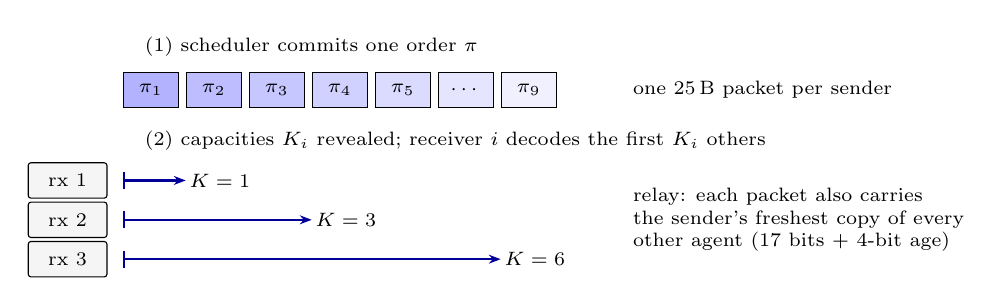
\begin{tikzpicture}[font=\scriptsize, pkt/.style={draw, minimum width=7mm, minimum height=4.5mm, inner sep=0pt},
  rx/.style={draw, rounded corners=1pt, minimum width=10mm, minimum height=4.5mm, fill=black!4}]
\node[anchor=west] at (-0.2,1.05) {(1) scheduler commits one order $\pi$};
\foreach \i/\lab in {0/$\pi_1$,1/$\pi_2$,2/$\pi_3$,3/$\pi_4$,4/$\pi_5$,5/$\cdots$,6/$\pi_9$}
  \node[pkt, fill=blue!\the\numexpr 30-4*\i\relax] (p\i) at (\i*0.8,0.5) {\lab};
\node[anchor=west] at (6.0,0.5) {one 25\,B packet per sender};
\node[anchor=west] at (-0.2,-0.15) {(2) capacities $K_i$ revealed; receiver $i$ decodes the first $K_i$ others};
\foreach \r/\k/\y in {1/1/-0.65,2/3/-1.15,3/6/-1.65}{
  \node[rx, anchor=east] (r\r) at (-0.55,\y) {rx $\r$};
  \draw[|-{Stealth[length=1.5mm]}, thick, blue!60!black] ($(p0.west)+(0,\y-0.5)$) -- ++(\k*0.8,0) node[right, inner sep=1pt, black] {$K=\k$};
}
\node[anchor=west, align=left] at (6.0,-1.15) {relay: each packet also carries\\ the sender's freshest copy of every\\ other agent (17 bits + 4-bit age)};
\end{tikzpicture}
\caption{The prefix-broadcast channel. A receiver with a small capacity hears only the head. Under a congestion-ranked
order the same senders stay in front, so low-ranked senders are rarely transmitted; relay spreads their last copies, which
then age.}
\label{fig:channel}
\end{figure}

Budgeted multi-agent communication is usually evaluated against agents trained without messages. We study a channel in
which that comparator turns out to be weak. One broadcast stream is committed per step. After it is committed, each
receiver learns how many packets it can decode, and it decodes the first $K_i$ of the stream (Figure~\ref{fig:channel}).
Capacities differ between receivers and change every step, as in layered and priority-encoded multicast~\cite{rlm,pet};
here the receivers are learned agents controlling traffic signals.

We measure communication against \emph{compiled silence}: a student distilled from the same full-information teacher that
receives no messages. On this channel, learned actors that use their deliveries lose even to a co-trained silent actor,
and compiled silence is stronger still. We identify three contributing mechanisms of the failure and a repair inside the
unchanged packet and byte contract: relay tables in every packet, and an age-first stream order. Relay alone gives every
receiver a copy of every sender, but under the congestion order those copies are old, and a student trained at iid
capacity fails at low capacity; age-first ordering makes the copies fresh without retraining.
The mathematics of the channel explains why this repair is close to what any order can achieve. The decoded sets are
prefixes of one order and therefore nested, so one receiver always holds everything transmitted in a step, and a head
chosen among such receivers brings every other receiver, one step later, up to what it knew.

\paragraph{Contributions.}
\begin{itemize}
\item A MARL evaluation of the receiver-dependent prefix channel, with explicit byte accounting and an oracle-access audit
(Sections~\ref{sec:model} and~\ref{sec:exp}).
\item Compiled silence as the comparator for deployment-time communication, with controls for distillation, compute,
teacher information and the comparator's own seed variance (Section~\ref{sec:res-bar}).
\item A failure analysis in which each alternative hypothesis is tested by a rule written before its result
(Section~\ref{sec:res-mech}).
\item A pre-specified test showing that, in this channel, relay under the congestion order gives coverage without freshness
and that age-first ordering closes the gap for students trained at iid capacity (Section~\ref{sec:res-fix}).
\item Freshness results for the channel: an injection bound for age-first ordering, the minimum mean injection age for a
given stream length, a one-step bound for relay with a covering head, and monotonicity in capacity
(Section~\ref{sec:fresh}); with replica and closed-loop checks, including a heterogeneous-capacity test whose outcome was
predicted before the run (Section~\ref{sec:res-math}).
\end{itemize}

\section{Related work}\label{sec:related}
\paragraph{When learned communication fails.} Chauhan and Bera~\cite{chauhan2026} find, at matched 2-bit rates over 25
seeds, that learned senders are often indistinguishable from silence while engineered senders succeed, and localise the
failure in protocol discovery. CAIC~\cite{caic} models a shared channel as a queue and finds that stale messages under
delay can be worse than none. I2C~\cite{i2c} notes that broadcast redundancy can impair learning. In the channel studied
here the payloads are engineered summaries, and staleness arises from which packets each receiver decodes.
\paragraph{Communication under budgets.} SchedNet~\cite{schednet} learns who broadcasts, and IMAC~\cite{imac} learns
messages and schedules jointly. NDQ~\cite{ndq}, information-bottleneck and vector-quantised messages~\cite{ibvq},
event-triggered sending~\cite{etcnet} and Where2comm~\cite{where2comm} reduce bytes. CACOM~\cite{cacom} personalises
messages per receiver after a coarse broadcast. AH-VIB~\cite{ahvib} makes one message robust to truncation of its
dimensions to a prefix, and names learning which agent communicates at which slot as open. Here every receiver decodes a
prefix of one common ordered broadcast, and the order of senders in that stream is the object of study.
\paragraph{Multi-hop, global and delayed information.} Graph controllers imitate centralised experts from delayed $k$-hop
information~\cite{gama2022,tolstaya2019}; NeurComm propagates delayed global information in traffic control~\cite{neurcomm}.
Message chains (TEM~\cite{tem}), two-hop relays (AC2C~\cite{ac2c}), full-team recurrent chains (FCMNet~\cite{fcmnet}) and
low-diameter topologies with memory (ExpoComm~\cite{expocomm}) spread information further, and LMAC~\cite{lmac} designs
protocols under which every agent reconstructs the state uniformly. Delay-aware methods include DACOM~\cite{dacom},
CoDe~\cite{code}, VIL2C~\cite{vil2c}, which values delayed messages by their effect on the recipient's decision, and
CGDC~\cite{cgdc}, which separates communication gain from delay cost.
\paragraph{Freshness and scheduling.} All-to-all dissemination in which every node is both a source and a monitor and
broadcasts carry other nodes' states (piggybacking) goes back to vehicular safety messaging~\cite{kaul2011}, which also
defines the relay age; lower bounds on age, and schedules that attain them, are known when each transmission carries a
single status~\cite{farazi2019}. Here several senders are decoded per step, by prefix and with heterogeneous capacity, and
each packet carries its sender's whole table. Keeping every source fresh on a shared channel is age-of-information scheduling; in
symmetric broadcast networks the greedy highest-age-first policy is optimal~\cite{kadota2018}, and round-robin is
$O(1)$-competitive under packet management~\cite{jien2023}. Freshest-copy merging of timestamped relays is gossip, whose
age scaling with network size is analysed in~\cite{yates2021,selen2013}. Periodic per-source deadlines are pinwheel
scheduling, where every instance of density at most $5/6$ is schedulable~\cite{kawamura2024}. One broadcast for clients
with different needs is broadcast disks~\cite{broadcastdisks}. One order serving every cardinality is incremental
maximisation~\cite{bernstein2022,bienkowski2026}, and one sequence serving every house size within quota is house-monotone
apportionment~\cite{balinski1982}.
\paragraph{Information architecture and information structures.} Moeller and Krishnamachari~\cite{moeller2026} study the
trade-off between the scope and the age of a team's information in exogenous linear-quadratic environments, where the
delay is a given function of the scope and communication is not charged; what governs performance there is the
predictability of the optimal decision rather than of the state. Liu, You and Zhang~\cite{liu2026ltc} formalise learning to
communicate through information structures, with a cost on additional sharing, and Matni~\cite{matni2017} co-designs
communication delays with a distributed controller. Here the delay is produced by a byte-charged broadcast schedule, the
traffic state is endogenous, and the policies are learned.
\paragraph{Privileged teachers and communication-free students.} Centralised or privileged teachers are distilled into
decentralised students in CTDS~\cite{ctds}, PTDE~\cite{ptde}, HINT~\cite{hint}, communication-enhanced tutoring~\cite{tutoring},
KD-MARL~\cite{kdmarl} and MAGPO~\cite{magpo}, and into communication-free students in CoDiMAD~\cite{codimad}. These works
ask whether privileged training improves decentralised execution. Here the zero-byte student is the reference against
which runtime communication is credited: messages count only for what they add beyond the coordination compiled into a
zero-byte policy by the same teacher and recipe.
\paragraph{Traffic.} CityFlow~\cite{cityflow}; CoLight~\cite{colight}; UniComm~\cite{unicomm} (compact predictions of
neighbour impact); max pressure~\cite{varaiya2013}; MAPPO~\cite{mappo}; DAgger~\cite{dagger}.

\section{Methodology}\label{sec:method}
\subsection{The channel}\label{sec:model}
There are $m$ agents, each a sender and a receiver ($m=9$ intersections in E3), and decision steps $t=0,1,\dots$. At step
$t$ the scheduler commits an order $\pi_t$ of the senders, with $\mathrm{pos}_t(j)\in\{0,\dots,m-1\}$ the position of $j$.
Capacities $K_t(i)\ge1$ are then revealed, and receiver $i$ decodes the first $K_t(i)$ senders of $\pi_t$ other than itself.
\begin{lemma}[Threshold form]\label{lem:thr}
Let $r_t(i)=K_t(i)+\mathbf 1[\mathrm{pos}_t(i)<K_t(i)]$. The decoded set is
$S_t(i)=\{\,j\ne i:\mathrm{pos}_t(j)<r_t(i)\,\}$. \LEANC{LeanMarlPrefixThresholdV1.firstK\_eq\_threshold}
\end{lemma}
\emph{Proof.} The number of senders other than $i$ ahead of $j$ is $\mathrm{pos}_t(j)-\mathbf 1[\mathrm{pos}_t(i)<\mathrm{pos}_t(j)]$.
If $\mathrm{pos}_t(i)<K_t(i)$, the condition ``fewer than $K_t(i)$ ahead'' is $\mathrm{pos}_t(j)<K_t(i)+1$ for every $j$. If
$\mathrm{pos}_t(i)\ge K_t(i)$, it is $\mathrm{pos}_t(j)<K_t(i)$, since every $j$ behind $i$ already has $\mathrm{pos}_t(j)>K_t(i)$. $\square$

The transmitted set is $U_t=\bigcup_iS_t(i)$, a prefix of $\pi_t$. A profile is charged 25\,B per packet of that prefix
plus its description, as in the protocol (PROTOCOL\_HETERO\_v0), so the stream length $L_t=|U_t|$ sets the bytes. The
scheduler may use the payloads paid in earlier steps and their measurement times, a mirror of every receiver's cache, the
revealed capacities, the public topology and the actor code. Fresh states, counterfactual views and oracle rollouts are
used only as training labels or labelled diagnostics.

\subsection{Relay packets and the merge}\label{sec:relay}
Sender $k$'s 25\,B packet carries its own 17-bit summary (phase 4, elapsed 1, vehicles $2\times4$, waiting $1\times4$ bits)
and, for each other agent $j$, the 17 bits of the freshest summary of $j$ that $k$ holds plus a 4-bit age in steps
(saturated at 14; 15 means absent): $17+8\times21=185$ bits (it fits 200 bits iff $m\le9$,
\lean{LeanMarlStatLayoutV1.relay\_layout\_bits}), as in multi-hop
dissemination~\cite{tem,ac2c,fcmnet,expocomm}. Summary levels come from a codebook fitted on training
traffic.\NOTE{L-162, L-165 (byte-layout audit), L-174 (saturated ages).}

Write $T_t(i,j)$ for the measurement time of the copy of $j$ in $i$'s merged view after step $t$ ($-\infty$ if none), and
$C_t(i,j)$ for the last step at which $i$ decoded $j$ directly. The merge used in E3 is
\begin{equation}\label{eq:merge}
T_t(i,j)=\begin{cases} t & j\in S_t(i),\\ \max\big(C_t(i,j),\ \max_{k\in S_t(i)}T_{t-1}(k,j)\big) & \text{otherwise,}\end{cases}
\end{equation}
for $j\ne i$: a receiver keeps its direct copies and the tables of the packets it decodes in this step, but not the
relayed copies it received earlier. The age is $a_t(i,j)=t-T_t(i,j)$. Let $\ell_t(j)=\max\{s\le t:j\in U_s\}$ be $j$'s last
transmission and $f_t(j)=t-\ell_t(j)$ its injection age. No copy can be fresher than the last transmission:
$T_t(i,j)\le\ell_t(j)$, by induction on~\eqref{eq:merge}.

\subsection{Stream orders}\label{sec:orders}
\begin{itemize}
\item \emph{Congestion order} (the default): senders ranked by cached queue length.
\item \emph{Age-first}: the sender whose last transmission is oldest goes first, ties by index. This is highest-age-first
scheduling~\cite{kadota2018} applied to transmissions.
\item \emph{Hub head}: the head is a \emph{covering receiver} of the previous step (Definition~\ref{def:cover}), the rest age-first.
\item \emph{Mixture} $\beta$: age-first with probability $\beta$ at each step, the congestion order otherwise.
\item \emph{Deadline} $D$: the congestion order, with every sender whose worst relayed age is at least $D$ moved to the
front, oldest first.
\end{itemize}
Every order uses scheduler information only; the cap rule (stream limited to $c$ packets) applies under every order.

\subsection{Freshness under prefix decoding}\label{sec:fresh}
The statements below are proved on paper and in Lean (modules in \texttt{work/p13\_conjectures}, each with a satisfiability
witness). They compile with axioms within \{propext, Classical.choice, Quot.sound\}; the frozen gate run is pending, and
none is used as a theorem until it passes.
\begin{claim}[Injection bound]\label{cl:inj}
Under age-first ordering with $K_t(i)\ge1$ for all $i,t$, every sender is transmitted at least once in every $m$
consecutive steps, for every capacity sequence. \LEANC{LeanMarlAgeFirstInjectionV1.injection\_bound; on the prefix channel
LeanMarlChannelBridgeV1.injection\_bound\_prefix}
\end{claim}
\emph{Proof.} The head is decoded by every other receiver, so it is transmitted and its last-transmission time becomes the
newest. For a sender $j$ not transmitted at step $t$, every sender ranked before $j$ that is transmitted moves behind it,
and no sender behind $j$ can overtake it, since last-transmission times only increase. So $j$'s rank falls by at least one
per step until $j$ is the head, within $m-1$ steps. $\square$

Under a fixed (sticky) order, a sender outside every decoded prefix is never transmitted. The claim does not say that the
head visits every sender: with several packets transmitted per step and ties broken by index, the head concentrates on
a few senders (Section~\ref{sec:res-math}).

\begin{claim}[Injection floor]\label{cl:floor}
If at most $L$ senders are transmitted per step, then at every step $t\ge\lceil m/L\rceil$ the injection ages satisfy
$\#\{j:f_t(j)\le s\}\le(s+1)L$ for every $s$, hence
\[\frac1m\sum_jf_t(j)\ \ge\ F(m,L)=\frac1m\sum_{s\ge0}s\cdot\min\big(L,(m-sL)_+\big).\]
Age-first ordering with exactly $L$ transmissions per step attains $F(m,L)$ at every step after the first
$\lceil m/L\rceil$. \LEANC{LeanMarlInjectionFloorV1.injection\_floor, count\_recent; attainment only on an example,
floor\_attained\_example}
\end{claim}
\emph{Proof.} A sender with $f_t(j)\le s$ was transmitted in one of the $s+1$ steps $t-s,\dots,t$, each of which transmits at
most $L$ senders. Sorting the ages, the $r$-th smallest is at least $\lfloor(r-1)/L\rfloor$, and summing gives the bound. Under
age-first with $L$ transmissions per step, the $L$ oldest senders are transmitted at every step, so after the first
$\lceil m/L\rceil$ steps the sorted ages are exactly $0^{(L)},1^{(L)},\dots$, which attains the bound. $\square$

Since $T_t(i,j)\le\ell_t(j)$, no order makes the mean receiver age smaller than $F(m,L)$, and $L$ is fixed by the bytes
spent. $F(9,2)=16/9$, $F(9,3)=1$, $F(9,4)=2/3$.

\begin{definition}\label{def:cover}
A receiver $c$ \emph{covers} step $t$ if $U_t\setminus\{c\}\subseteq S_t(c)$: it decoded everything transmitted except its
own packet.
\end{definition}
\begin{lemma}[A covering receiver always exists]\label{lem:cover}
Any receiver with the largest threshold $r_t(i)$ covers step $t$; the same holds under the cap rule, with thresholds
$\min(r_t(i),c)$. \LEANC{LeanMarlRelayOneHopV1.prefix\_cover\_exists; LeanMarlChannelBridgeV1.capped\_cover\_exists}
\end{lemma}
\emph{Proof.} By Lemma~\ref{lem:thr}, $U_t=\{j:\mathrm{pos}_t(j)<\max_ir_t(i)\}$ up to the receivers' own packets, and
$S_t(c)=\{j\ne c:\mathrm{pos}_t(j)<r_t(c)\}$ with $r_t(c)=\max_ir_t(i)$. $\square$

This is where prefix decoding matters: the decoded sets are nested, so the best-informed receiver knows what every other
receiver decoded.

\begin{claim}[One-step freshness with a covering head]\label{cl:onehop}
Assume $K_t(i)\ge1$, the merge~\eqref{eq:merge}, and a head sequence $h_t$ such that $h_{t+1}$ covers step $t$ and
$h_{t+1}\ne h_t$. Then for every $t$:
\begin{itemize}
\item the head's table is as fresh as the network: $T_t(h_{t+1},j)=\ell_t(j)$ for all $j\ne h_{t+1}$;
\item every other receiver is at most one step behind: $f_{t+1}(j)\le a_{t+1}(i,j)\le1+f_t(j)$ for all $i\ne h_{t+1}$ and
$j\ne i$.
\end{itemize}
This holds for every capacity sequence, however unequal the capacities. \LEANC{LeanMarlRelayOneHopV1.head\_table\_fresh,
one\_hop, one\_hop\_age, witness\_one\_hop}
\end{claim}
\emph{Proof.} First part, by induction on $t$. If $j\in U_t$, then $j\in S_t(h_{t+1})$ because $h_{t+1}$ covers step $t$, so
$T_t(h_{t+1},j)=t=\ell_t(j)$. If $j\notin U_t$, then $\ell_t(j)=\ell_{t-1}(j)$, and $j\ne h_t$ because the head is transmitted.
Since $h_{t+1}\ne h_t$ decodes the head $h_t$, \eqref{eq:merge} gives $T_t(h_{t+1},j)\ge T_{t-1}(h_t,j)=\ell_{t-1}(j)$ by the
induction hypothesis. Equality follows from $T\le\ell$. At $t=0$ both sides are $-\infty$ for $j\notin U_0$.

Second part. The upper bound on $T$ is $T\le\ell$. If $j\in S_{t+1}(i)$, then $T_{t+1}(i,j)=t+1\ge\ell_t(j)$. Otherwise $i$
decodes the head $h_{t+1}$ and $j\ne h_{t+1}$, so $T_{t+1}(i,j)\ge T_t(h_{t+1},j)=\ell_t(j)$. $\square$

Relay therefore turns unequal capacities into a cost of at most one step relative to the injection ages of the schedule
used. Without relay, a receiver with $K=1$ hears one sender per step directly. The head choice is a trade-off: a covering
head takes the first slot away from the oldest sender, so the injection ages can exceed the floor of Claim~\ref{cl:floor}
(Section~\ref{sec:res-math}).

\begin{claim}[Relay memory is redundant under a covering head]\label{cl:memory}
Under the hypotheses of Claim~\ref{cl:onehop}, a persistent (gossip) merge that also keeps a receiver's earlier relayed
copies gives exactly the same table as~\eqref{eq:merge}, for every receiver other than the head, at every step.
\LEANC{LeanMarlRelayMemoryV1.memory\_redundant}
\end{claim}
\emph{Proof.} Off the direct branch both tables are at most $\ell_t(j)$ (no copy is fresher than the last transmission up to
$t$), and by Claim~\ref{cl:onehop} the transient one is at least $\ell_t(j)$; the persistent one keeps more, so it lies in
between. $\square$

\begin{claim}[Monotonicity in capacity for a fixed order sequence]\label{cl:mono}
Fix the orders $\pi_t$. If $K_t(i)\le K'_t(i)$ for all $i,t$, then $T_t(i,j)\le T'_t(i,j)$ for all $i,j,t$. \LEANC{LeanMarlRelayMonotoneV1.freshness\_mono\_capacity; LeanMarlChannelBridgeV1.threshold\_mono}
\end{claim}
\emph{Proof.} By Lemma~\ref{lem:thr}, $S_t(i)\subseteq S'_t(i)$, and~\eqref{eq:merge} is monotone in the decoded set and in the
previous tables; induct on $t$. $\square$

Claims~\ref{cl:floor}--\ref{cl:mono} concern information. A fixed nonlinear policy's return need not be monotone in it.

\begin{remark}[Phase-lock without relay]\label{rem:lock}
With raw one-sender packets, constant capacity $K$, age-first ordering and ties broken by index, some pairs are never
covered in steady state. When $L=K+1$ divides $m$, the never-covered share is $(m-L)/(L(m-1))$: 25\% at $m=9$, $K=2$.
Non-divisible cases also lock, at smaller shares, and random tie-breaking removes the lock. The instance $m=9$, $K=2$
(18 of 72 pairs never covered, at every step) is proved by kernel computation
(\lean{LeanMarlPhaseLockV1.never\_covered\_count}, \lean{never\_covered\_forever}); the general formula and the other
cases are checked numerically (Section~\ref{sec:res-math}).
\end{remark}

\begin{claim}[Decision lifetime]\label{cl:life}
Let $q_f$ and $q_r$ be an actor's logits on the fresh complete view and on its relay view. If $\gamma=q_f(a^\ast)-\max_{a\ne
a^\ast}q_f(a)>2\inf_c\|q_r-q_f-c\mathbf1\|_\infty$, then the relay action is $a^\ast$. The argmax step is
\lean{LeanMarlDecisionCertificateV1.argmax\_stable} (\PROVED); the shift-invariant form and the composition with an age
bound are \LEANC{LeanMarlDecisionLifetimeV1.relay\_action\_equals\_fresh}. The dependence of the perturbation on age is
measured, not derived.
\end{claim}

\subsection{Policies and comparators}\label{sec:policies}
A flat actor concatenates eight sender blocks (fresh flag, heard flag, age, phase, elapsed, vehicles and waiting per
approach, static topology) with its own state. A set actor applies one shared encoder to each present sender block and
mean-pools over present senders. Both are trained by MAPPO with a centralised critic~\cite{mappo}. The teacher is a set
actor trained with full, fresh delivery. Students are trained by DAgger~\cite{dagger}: a student acts on its own
deployment input, and the teacher labels its states from the counterfactual full view (a training-only oracle), with the
teacher mixture decaying from 1 to 0 over the first half of 500 iterations. The comparators are:
\begin{itemize}
\item \emph{compiled silence}, the teacher distilled into a policy with no message input, and a second one per teacher
that differs only in its seed;
\item \emph{set\_none}, a set actor co-trained with no messages;
\item \emph{maxq}, serving the approach with the largest queue;
\item \emph{FO}, the teacher deployed with a fresh-only receiver;
\item \emph{BYTEBUDGET}, a reference in a byte-limited channel (receiver capacity $25K_i$ bytes spent on 3\,B packets).
\end{itemize}
The primary comparison holds the teacher and the DAgger recipe fixed: the relay student and the zero-byte student differ
only in their deployment input. What compiled silence can achieve is characterised by the obstruction law of the corpus,
instantiated at local observations: a zero-byte policy is acceptable everywhere iff no obstruction lies inside a local
observation class, it fails on such an obstruction, and a finer (message-augmented) observation keeps any zero-byte
guarantee \LEANC{LeanMarlCompiledSilenceV1.zero\_byte\_safe\_iff, zero\_byte\_fails\_on\_obstruction, messages\_keep\_safety;
from LeanUnifiedObstructionOrderV1 (\PROVED)}. The counting identity behind the V-U pitfall is
\lean{LeanMarlCompiledSilenceV1.agreement\_split} and \lean{split\_is\_tautological}.

\section{Experiments}\label{sec:exp}
\paragraph{Testbed.} CityFlow $3\times3$ grid~\cite{cityflow}, headways 8 and 16\,s, 26 decision steps 10\,s apart; the metric
is total queue (waiting) per episode. Capacity conditions:
\begin{itemize}
\item iid: $K_i\sim U\{1,\dots,7\}$ per receiver and step;
\item cap4: iid capacities with the stream capped at 4 packets;
\item low: $K_i\sim U\{1,2,3\}$;
\item constant $K$ (frontier study);
\item rich7: at each step one receiver, drawn from a generator seeded by the episode, decodes 7 packets and the others 1.
\end{itemize}
The average step costs 188.7\,B (iid), 100\,B (cap4), about 94\,B (low) and about 190\,B (rich7). Transport delay is zero,
so the ages studied here come only from which packets are decoded.
\paragraph{Panels.}
\begin{itemize}
\item Development: traffic seeds 901--964 $\times$ both headways (128 episodes).
\item Pre-specified test panels: unused seed blocks between 2001 and 2664, each used once. Each protocol was written, and
its hash recorded in the audit ledger, before any run on its panel.
\item Reserved test: seeds 1301--1316, untouched.
\end{itemize}
\paragraph{Statistics.} Comparisons are paired by episode and reported as the ratio of summed waiting minus one, with 95\%
bootstrap intervals over traffic seeds (both headways resampled together, 4000 draws). These intervals hold the trained
models fixed and do not include training-seed variation, which is reported across teacher/student pairs. The rule of the
pre-specified relay test requires every one of six upper bounds to be below zero. This is an intersection--union test:
each one-sided test at level 2.5\% gives the conjunction level at most 2.5\% without multiplicity
adjustment~\cite{berger1982} \LEANC{LeanMarlStatLayoutV1.intersection\_union\_test}. The six intervals are not a joint
confidence region.
\paragraph{Audits.} Every evaluation runs a per-step oracle-access audit, and every oracle call inside a deployable path
raises. Bytes are charged as in the protocol. Two further checks run at every relay step:
\begin{itemize}
\item the scheduler's mirror of the relay tables must equal the receivers' merged views;
\item each new evaluator must reproduce the previous one row for row where their options coincide.
\end{itemize}
Each diagnostic hypothesis has a reading rule written before its result, and negative results are reported.
\paragraph{Probes.} To test the mechanism chain, a probe replays the relay student's closed-loop rollouts and records, per
receiver-step:
\begin{itemize}
\item the student's logits on its relay view and on the counterfactual fresh complete view;
\item the teacher's actions (raw and 3\,B inputs) and a zero-byte student's action;
\item the relayed ages and the capacities.
\end{itemize}
Probe rows must match the evaluator's rows exactly. A second zero-byte student is probed on the same states as a
same-information null. The traffic-free replica of the channel uses the E3 prefix sets and the E3 mirror of the merge.
\paragraph{Predictions from other models.} Several checks take the shape of a result proved in another model and measure
it here:
\begin{itemize}
\item frozen-surrogate starvation and repair, against the mixture $\beta$ (V-A);
\item signed versus monotone budget regimes, against the constant-$K$ frontier (V-S);
\item certificate lifetime and margin, against age and margin (V-F);
\item decide-not-identify, against 3\,B compression (V-B);
\item obstruction floors, against the null split (V-U);
\item quota tracking, against rotation as apportionment (V-Q).
\end{itemize}
The source results are proved in their own models; here they supply predictions only.

\section{Results}\label{sec:results}
\subsection{Compiled silence is a stronger bar}\label{sec:res-bar}
\paragraph{Learned actors that use their messages lose to silence.} On the development panel, a flat actor trained without
messages has $8.0\%$ $[7.4,8.6]$ less waiting than the committed-prefix system of five flat prefix-trained actors, and less
than each of them ($5.6$ to $10.5\%$). Doubling the prefix actor's training leaves it $6.3\%$ $[5.3,7.4]$ worse. Max pressure
as implemented has about 14\% more waiting than the same rule without its message-fed terms (max-queue). An earlier line of
work that scheduled messages for frozen prefix-trained actors found no legal selector better than the committed prefix
(Appendix~\ref{app:history}).\NOTE{L-78, L-81, L-105, L-109, L-113--L-116.}
\paragraph{The zero-byte student.} Over five training seeds it has $3.5\%$ $[2.2,4.9]$ less waiting than set\_none, and less on
every seed. The same DAgger recipe with a silent teacher gives $+0.2$, $-0.2$ and $+0.2\%$ (three seeds). 500 more PPO
iterations for set\_none give $+2.0\%$. The gain grows with the teacher's information: $\approx0$ for a silent teacher,
$-2.3/-0.9\%$ for a prefix-message teacher and $-3.2/-6.3\%$ for a full-information teacher. A second zero-byte student per
teacher differs from the first by $-0.26\%$ $[-1.08,+0.55]$ (seed 0) and $-1.20\%$ $[-1.99,-0.49]$ (seed 1), so one student
per teacher can understate the bar by about one percent.\NOTE{L-147--L-160 (two-level bootstrap for the five seeds), L-178.}
\paragraph{Designs inside the packet channel} (pre-specified panels, both seeds required):
\begin{center}\small
\begin{tabular}{@{}lccl@{}}
\toprule
design & seed 0 & seed 1 & verdict\\
\midrule
FO vs set\_none & $-3.0\%$ & $-5.2\%$ & passes against the weak bar\\
FO vs the zero-byte student & $+1.3\%$ & $+2.1\%$ & the student is better\\
fresh-only student vs the zero-byte student & $-0.8\%$ (fail) & $-4.0\%$ & seed-dependent\\
set\_fresh vs the zero-byte student & $-2.0\%$ & $+7.2\%$ (fail) & seed-dependent\\
\bottomrule
\end{tabular}
\end{center}
\NOTE{L-127, L-129, L-138, L-140, L-141, L-144--L-146, L-150.}

\subsection{Three contributing mechanisms}\label{sec:res-mech}
\paragraph{Sparse sender exposure.} A flat actor trained with full delivery keeps 79--85\% of its full-information gain when
5--7 of 8 senders are present, but falls below the silent actor under the protocol's capacity process ($+4.2$ and $+1.3\%$),
where about half the senders are absent. Mean pooling over present senders degrades gracefully. Irrelevant input dimensions
(H1), stale content alone (H5) and weight sharing without pooling (H3) are refuted by their rules, and doubling the width
(H7) does not close the gap.\NOTE{L-132, L-133, L-135, L-142, L-157.}
\paragraph{Stale cached copies.} The full-information set teacher, deployed with its stale cached blocks, is no better than
set\_none ($-0.1\%$ $[-1.0,+0.9]$). Dropping stale blocks (FO) recovers 59\% of the full-information gain.\NOTE{L-124,
L-125, L-127, L-138.}
\paragraph{Starvation under the congestion order.} In the replica, a sticky ranking at cap4 leaves 40--46\% of (receiver,
agent) pairs never covered. With relay in CityFlow the pairs are covered, but the mean relayed age is 5.4 steps and 45\% of
copies are at least 4 steps old under cap4 and low. Age-first ordering gives 0.8--1.4 steps and 0--5\%.\NOTE{L-168, L-177.}
We have not tested whether the three mechanisms interact beyond adding up.

\subsection{Coverage by relay, freshness by age-first ordering}\label{sec:res-fix}
\begin{figure}[t]
\centering
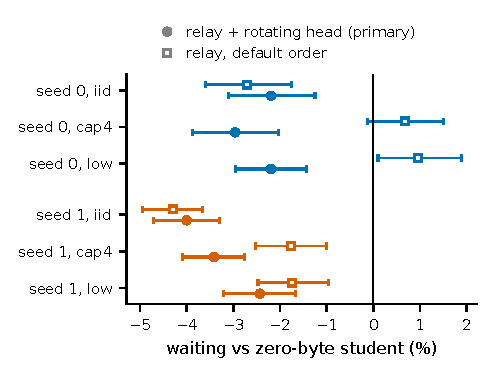
\includegraphics[width=0.62\linewidth]{fig_prereg.pdf}
\caption{Pre-specified panel 2601--2664 (128 episodes, used once): total waiting against the same-seed zero-byte student,
95\% bootstrap over traffic seeds. Filled: relay under age-first ordering (primary). Hollow: relay under the congestion
order (secondary). \NOTE{from e3\_relayrot\_panel\_report\_20260930.json; L-175.}}
\label{fig:prereg}
\end{figure}
\paragraph{Relay under the congestion order.} On the development panel, relay beats the zero-byte student at iid by $3.3\%$
$[2.5,4.2]$ and $4.0\%$ $[3.1,5.0]$, and without messages the same student is $4.8\%$ worse than the zero-byte student, so it
uses them. At low capacity the advantage disappears: seed 0 is $+0.9\%$ (cap4) and $+0.4\%$ (low). Against the second
zero-byte student it is $+1.21\%$ $[+0.28,+2.20]$ and $+0.61\%$ $[-0.14,+1.40]$ (seed 0) and $-0.42\%$ $[-1.22,+0.44]$ and
$-0.20\%$ $[-1.08,+0.72]$ (seed 1): a loss or a tie in all four low-capacity cells.\NOTE{L-163, L-169, L-174, L-178.}
\paragraph{Age-first ordering.} On the development panel it restores the advantage at cap4 ($-2.3$ / $-4.1\%$) and low
($-2.8$ / $-3.0\%$). The iid cost is $+0.3$ / $+0.9\%$, not significant. Against the second zero-byte student it wins in all six
cells ($-2.80$, $-2.01$, $-2.55\%$ for seed 0; $-1.99$, $-2.98$, $-1.78\%$ for seed 1; every upper bound below zero).\NOTE{L-169,
L-174, L-178.}
\paragraph{Pre-specified test.} The primary endpoint is relay under age-first ordering against the same-seed zero-byte
student, on panel 2601--2664; all six upper bounds had to be below zero (Figure~\ref{fig:prereg}).
\begin{center}\small
\begin{tabular}{@{}lccc@{}}
\toprule
& iid (189\,B/step) & cap4 (100\,B/step) & low ($\approx94$\,B/step)\\
\midrule
seed 0 & $-2.19\%$ $[-3.10,-1.25]$ & $-2.96\%$ $[-3.87,-2.04]$ & $-2.19\%$ $[-2.95,-1.43]$\\
seed 1 & $-4.00\%$ $[-4.71,-3.30]$ & $-3.41\%$ $[-4.09,-2.75]$ & $-2.43\%$ $[-3.20,-1.67]$\\
\midrule
\multicolumn{4}{@{}l}{\emph{secondary: relay under the congestion order}}\\
seed 0 & $-2.71\%$ & $+0.68\%$ $[-0.12,+1.50]$ & $+0.96\%$ $[+0.10,+1.88]$\\
seed 1 & $-4.29\%$ & $-1.76\%$ & $-1.74\%$\\
\bottomrule
\end{tabular}
\end{center}
The primary rule is met in all six cells. On the same panel relay under age-first ordering also beats set\_none by
5.7--10.1\% and max-queue by 22.5--26.2\%; the byte-budget reference gives $-4.0$ / $-4.5\%$. The test used one zero-byte
student per teacher and two teacher/student pairs.\NOTE{L-173 (protocol hash c7467697\dots), L-175.}
\paragraph{Reserved ten-seed test}\label{sec:res-ten} (panel 2701--2764, used once; protocol written before any run on it).
Ten teacher/student pairs, relay students trained under age-first ordering, against each pair's zero-byte student. The
statistic per condition is the mean over the ten pairs of the paired waiting ratio minus one; its interval resamples the
pairs and then the traffic seeds within each pair (4000 draws); the rule required all three upper bounds below zero.
\begin{center}\small
\begin{tabular}{@{}lccc@{}}
\toprule
& iid & cap4 & low\\
\midrule
age-first, vs same-seed zero-byte student & $-2.29\%$ $[-3.25,-1.39]$ & $-2.04\%$ $[-3.03,-1.10]$ & $-1.26\%$ $[-2.08,-0.50]$\\
\multicolumn{4}{@{}l}{\emph{secondary}}\\
age-first, vs replicate zero-byte student & $-2.11\%$ $[-3.01,-1.25]$ & $-1.86\%$ $[-2.78,-0.93]$ & $-1.08\%$ $[-1.88,-0.31]$\\
congestion order, vs same-seed student & $-2.00\%$ $[-2.87,-1.17]$ & $+0.15\%$ $[-0.84,+1.10]$ & $+0.38\%$ $[-0.57,+1.36]$\\
\bottomrule
\end{tabular}
\end{center}
The rule is met. Per pair the effect ranges from $-4.6\%$ to $-0.2\%$ (mean over conditions); three of the ten pairs are
not individually below zero in most cells. Under the congestion order the advantage disappears at cap4 and low, as the
freshness analysis predicts (Section~\ref{sec:fresh}). Across pairs the effect correlates with the byte-budget headroom of
the same teacher (Spearman $0.87$, nine pairs).\NOTE{PROTOCOL\_E3\_TEN\_SEEDS\_20260930 (hash 4bb1ab17\dots); report
scripts/MARL\_e3\_ten\_seed\_panel\_report.py; L-201, L-202, L-203 (comparator, leakage and provenance checks).}
\paragraph{Ablations} (development, against the same-seed zero-byte student):
\begin{itemize}
\item MAPPO from scratch on relay inputs instead of distillation is $+2.0$ / $+4.5\%$ worse;
\item a head chosen for the freshest table (``bass'') equals age-first ordering at iid, cap4 and low;
\item the deadline order does not dominate for any $D\in\{2,3,4,6\}$ under the rule written before the run. It is worse than
age-first at low capacity ($+0.7$ to $+1.4\%$) and at cap4 for seed 1 ($+1.3$ to $+1.7\%$), and worse than the congestion
order at iid for seed 1 ($+0.7$ to $+1.0\%$).
\end{itemize}
\NOTE{L-166, L-169, L-178.}
\paragraph{Other students and other repairs (development; same-seed bar $Z$ and replicate $Z'$).}
\begin{itemize}
\item \emph{Replication.} Relay students with the corrected 185-bit layout, trained independently under the congestion order
at iid, reproduce the pattern: under the congestion order they fail at low capacity (seed 1: $+0.97\%$ $[+0.04,+1.84]$), and
under age-first ordering every cell has an upper bound below zero against both $Z$ and $Z'$.
\item \emph{Training at low capacity} (two seeds). A relay student trained at low capacity under the congestion order beats both bars at
cap4 and low without age-first ordering ($-3.4$ / $-2.9\%$ and $-4.0$ / $-4.2\%$, every upper bound against $Z'$ below
$-1.7$). It is weaker at iid and worse under age-first ordering (low: $-0.27\%$ $[-1.18,+0.72]$ and $-0.51\%$): copies
fresher than those it was trained on hurt it. The failure of iid-trained students under the congestion order is therefore
partly a shift in the age distribution between training and deployment. Age-first ordering removes it at deployment,
and training at the target capacity is an alternative.
\item \emph{A decision-sensitivity codebook.} A relay student whose summaries allocate bits by the teacher's decision
sensitivity (8 levels) beats both bars in all twelve cells, under both orders, for seeds 0 and 1. It does not remove the
order effect in general: on seeds 3--5 it loses to the zero-byte student under the congestion order at cap4 or low (seed 3,
low: $+1.57\%$ $[+0.82,+2.41]$; seed 4: $+0.91\%$, $+2.34\%$; seed 5: $+1.23\%$, $+1.07\%$, all lower bounds above zero), so
the robustness holds on two of five seeds. With 12 levels it holds for one seed of two: seed 1 fails under the congestion
order at cap4 and low ($+0.05\%$, $-0.11\%$), while age-first ordering wins in all six cells.\NOTE{L-184, L-187, L-203.}
\end{itemize}
\NOTE{L-184.}
\begin{figure}[t]
\centering
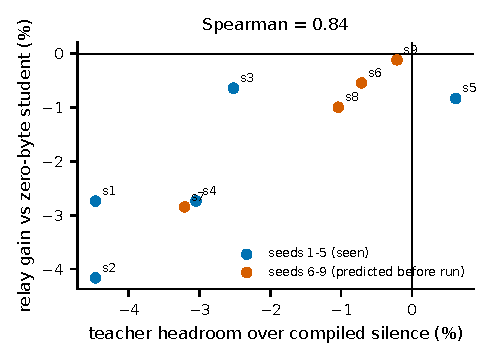
\includegraphics[width=0.55\linewidth]{fig_seeds.pdf}
\caption{Ten teacher/student pairs (development): relay under age-first ordering against each pair's zero-byte student
(mean of iid, cap4 and low), against the teacher's headroom over compiled silence in the byte-limited reference. Orange
points were predicted before their runs (L-179). \NOTE{e3\_seed\_prediction\_report\_20260930.json; L-185.}}
\label{fig:seeds}
\end{figure}
\paragraph{Ten training seeds and a prediction recorded before the run} (development; Figure~\ref{fig:seeds}).
\begin{itemize}
\item Relay students trained under age-first ordering, against their own zero-byte students, gain $-2.2$, $-2.7$, $-4.2$,
$-0.6$, $-2.7$, $-0.8$, $-0.5$, $-2.9$, $-1.0$ and $-0.1\%$ for seeds 0--9 (mean of iid, cap4 and low; overall mean
$-1.8\%$).
\item Before seeds 6--9 were evaluated, we recorded three predictions from the teacher's headroom over compiled silence
in the byte-limited reference: seed 7 would gain most among seeds 6--9; seeds 6, 8 and 9 would each gain less than
$1.5\%$; and the rank correlation over all seeds would be at least 0.5.
\item All three held, with a rank correlation of 0.84.
\end{itemize}
Runtime communication pays, here, in proportion to the information the teacher holds beyond what compiles into a
zero-byte policy. Where that headroom is below 1\%, the relay gain is at most 1\%.\NOTE{L-179, L-185.}
\TODO{a pre-specified test with these ten pairs and two-level uncertainty.}
\paragraph{Reference: a byte-limited channel.} Where receiver capacity is counted in bytes, 3\,B summaries from the raw
teacher beat the zero-byte student on 5/5 seeds by $3.6\%$ $[2.7,4.5]$, and by $2.5\%$ $[1.4,3.6]$ over eight seeds. The
result holds on three pre-specified panels, under unseen demand, with a refitted codebook and up to 25\% packet
loss.\NOTE{L-131, L-144, L-151, L-156, L-157, L-159, L-160, L-170.}

\subsection{The channel mathematics in the replica and in CityFlow}\label{sec:res-math}
\begin{figure}[t]
\centering
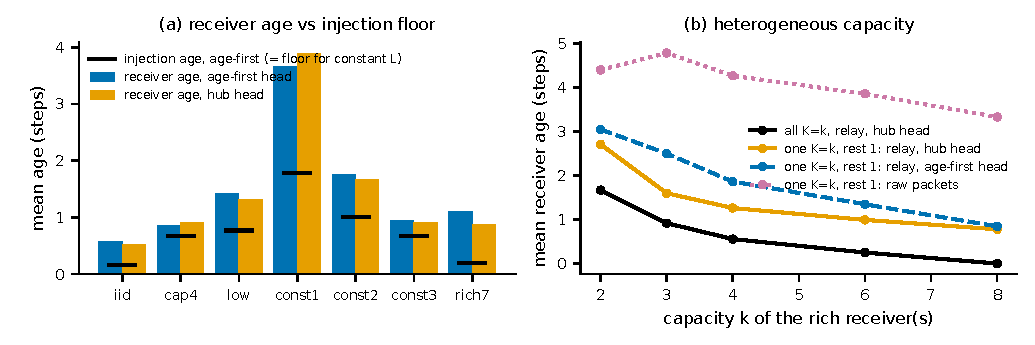
\includegraphics[width=\linewidth]{fig_math.pdf}
\caption{Traffic-free replica with the E3 prefix sets and merge. (a) Mean receiver age under the age-first and hub heads
against the injection floor $F(m,L)$ of Claim~\ref{cl:floor}, for each capacity process. (b) One rich receiver ($K=k$, the
others $K=1$) against all receivers $K=k$: relay with the hub head stays within about one step of the homogeneous
network, raw packets do not. \NOTE{scripts/MARL\_e3\_math\_replica.py $\to$ e3\_math\_replica\_20260930.json; L-181.}}
\label{fig:math}
\end{figure}
\paragraph{Replica checks of Section~\ref{sec:fresh}} (Figure~\ref{fig:math}):
\begin{itemize}
\item \emph{Injection floor.} Age-first ordering attains $F(9,L)$ exactly for constant transmission counts: 1.78, 1.00 and
0.67 steps for $L=2,3,4$.
\item \emph{One-step bound.} With a covering head, $f_{t+1}(j)\le a_{t+1}(i,j)\le1+f_t(j)$ holds in every one of $3.6\times10^5$
checks per capacity process (iid, low, constant $K=1$, rich7). As a control that can fail, the age-first head violates it in
7--38\% of the checks.
\item \emph{Heterogeneous capacity.} With one rich receiver ($K=k$, the others 1), relay with the hub head is within 0.7--0.8
step of the homogeneous network with the same capacity for $k=3$--8, and 1.0 step for $k=2$; raw packets are 1.7--3.2 steps
staler than relay with the hub head.
\item \emph{The head trade-off.} The hub head can slow injection: at constant $K=1$ its injection age is 3.11 steps against
the floor 1.78, and its mean receiver age (3.89) exceeds age-first's (3.67). Under iid, low and rich7 capacities the hub
head lowers the mean receiver age (0.53, 1.31 and 0.88 against 0.58, 1.42 and 1.11).
\item \emph{Relay memory.} Keeping previously relayed copies (gossip) changes mean ages by at most 0.02 step, as nestedness
predicts.
\item \emph{Head concentration and phase-lock.} Under iid capacities, age-first ordering gives 80\% of head slots to three
senders, and about 3 of 9 senders never head an episode. The phase-lock share of Remark~\ref{rem:lock} matches the formula
in all 12 divisible cases with $4\le m\le13$; random ties remove every lock.
\end{itemize}
\NOTE{L-180, L-181.}
\begin{figure}[t]
\centering
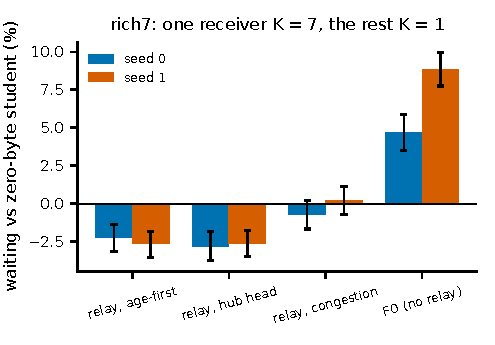
\includegraphics[width=0.55\linewidth]{fig_rich.pdf}
\caption{rich7 (one receiver decodes 7 packets per step, the others 1), development panel, against the same-seed zero-byte
student, 95\% intervals. \NOTE{L-182.}}
\label{fig:rich}
\end{figure}
\paragraph{A heterogeneous-capacity test, predicted before the run} (rich7, development; Figure~\ref{fig:rich}). Three predictions were recorded
before any run: relay with age-first ordering beats compiled silence (P1); the hub head is at least as good as age-first
(P2); and the gap between FO and relay widens relative to iid (P3).
\begin{itemize}
\item P1: $-2.24\%$ $[-3.11,-1.39]$ and $-2.63\%$ $[-3.51,-1.80]$.
\item P2: hub minus age-first is $-0.58\%$ $[-1.31,+0.17]$ and $+0.05\%$ $[-0.70,+0.81]$, a weak result. The freshest-table head
produces rows identical to the hub head, as the replica predicts for this condition.
\item P3: FO minus relay grows from $+3.1$ to $+7.1\%$ (seed 0) and from $+5.5$ to $+11.8\%$ (seed 1).
\end{itemize}
Relay under the congestion order again fails to beat the bar ($-0.70\%$ $[-1.66,+0.23]$, $+0.24\%$).\NOTE{L-181, L-182.}

\subsection{Probes of the mechanism chain}\label{sec:res-probe}
\begin{figure}[t]
\centering
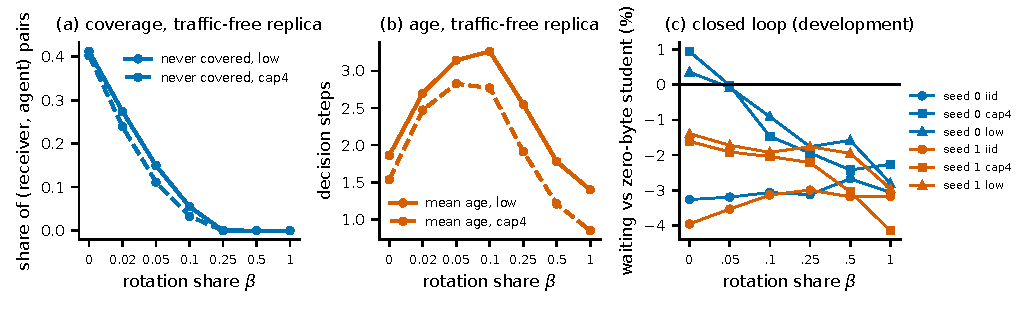
\includegraphics[width=\linewidth]{fig_va.pdf}
\caption{V-A. With probability $\beta$ the order is age-first, otherwise the congestion order. (a, b) Replica with relay:
the never-covered share falls with no threshold, but the mean age first rises and falls only once age-first ordering
dominates. (c) Closed loop, development panel, against the zero-byte student. \NOTE{L-176, L-177.}}
\label{fig:va}
\end{figure}
\paragraph{V-A: coverage is not freshness} (Figure~\ref{fig:va}). At low capacity the never-covered share falls from 0.41 to
0.27 at $\beta=0.02$ and to 0 at $\beta=0.25$, while the mean age rises from 1.9 to 3.3 steps at $\beta=0.1$ before falling to 1.4
at $\beta=1$. In closed loop, seed 0 improves already at $\beta=0.05$ at cap4 ($-0.96\%$ $[-1.53,-0.43]$ against $\beta=0$). Seed 1 is
nearly flat until $\beta\ge0.5$, and its iid cost is significant at $\beta=0.1$ and $0.25$ ($+0.85$, $+0.99\%$). Newly covered
but stale copies pay little; the repair pays when coverage is also fresh.

\begin{figure}[t]
\centering
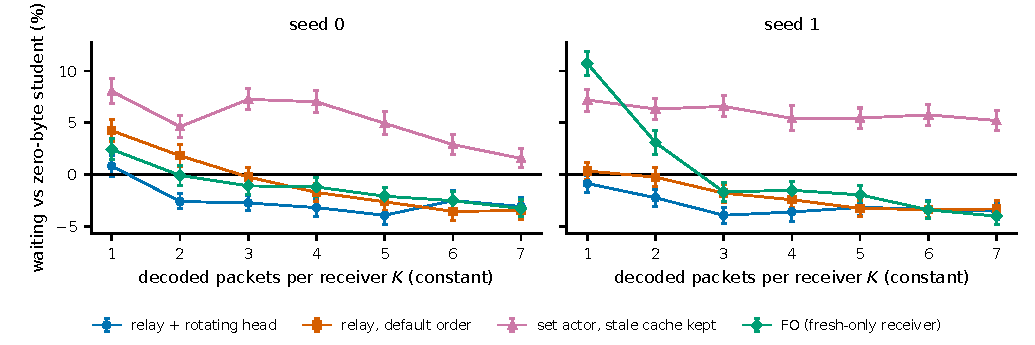
\includegraphics[width=\linewidth]{fig_vs.pdf}
\caption{V-S. Constant capacity $K$, development panel, against the zero-byte student (95\% intervals). \NOTE{L-177.}}
\label{fig:vs}
\end{figure}
\paragraph{V-S: the capacity frontier} (Figure~\ref{fig:vs}; exploratory). Relay under the congestion order and FO are
monotone on both seeds. The stale-kept set actor is non-monotone on seed 0 ($K=2\to3$), flat on seed 1, and never beats the
zero-byte student. Relay under age-first ordering wins from $K=2$ (seed 0) and $K=1$ (seed 1), with one significant
violation of monotonicity on seed 0 ($K=5\to6$). Information is monotone in $K$ for a fixed order (Claim~\ref{cl:mono}), but
the measured waiting is not always.

\begin{figure}[t]
\centering
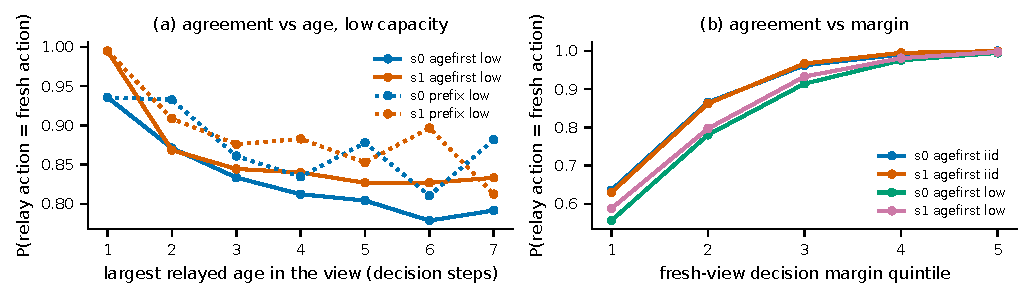
\includegraphics[width=\linewidth]{fig_vf.pdf}
\caption{V-F. Agreement of the relay-view action with the fresh-complete-view action on the relay student's own rollouts
(parity 128/128 with the evaluator), against the largest relayed age (a, low capacity) and the fresh margin (b).
\NOTE{L-177.}}
\label{fig:vf}
\end{figure}
\paragraph{V-F: age and margin} (Figure~\ref{fig:vf}). Agreement rises with the fresh margin from $\approx0.6$ in the lowest to
$\approx1.0$ in the highest quintile. Under age-first ordering it falls with the relayed age (0.94, 0.87, 0.83, 0.81, 0.80,
0.78 at ages 1--6, seed 0, low); under the congestion order it is not monotone, because the largest age is often that of a
starved sender. A certificate of the form of Claim~\ref{cl:life}, with a linear age term fitted on half the traffic seeds, is
sound on the other half ($\ge0.9997$) and covers 0--23\% of decisions.
\paragraph{V-B: compression.} 3\,B summaries change the teacher's own decision on 1.3--2.3\% of receiver-steps, almost all in the
smallest-margin quintile (7--11\% there, $\le0.3\%$ elsewhere).\NOTE{L-177.}

\begin{figure}[t]
\centering
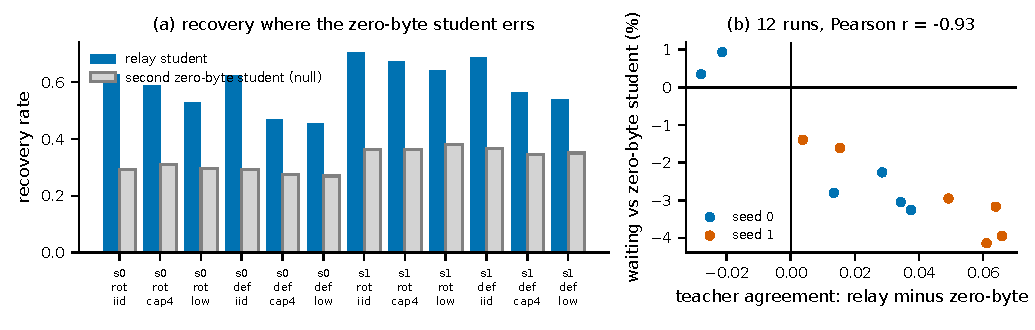
\includegraphics[width=\linewidth]{fig_vu.pdf}
\caption{V-U. (a) Where the zero-byte student $Z$ departs from the teacher, the share on which the relay student (blue) or a
second zero-byte student $Z'$ with the same local information (grey) takes the teacher's action; rot = age-first,
def = congestion order. (b) Net teacher agreement against waiting relative to $Z$, twelve conditions sharing two
teacher/student pairs. \NOTE{L-178.}}
\label{fig:vu}
\end{figure}
\paragraph{V-U: where messages move decisions} (Figure~\ref{fig:vu}). Conditioning on the steps where $Z$ departs from the
teacher and observing that another policy agrees more often there is true by construction. The comparison that carries
information is against $Z'$ on the same states:
\begin{itemize}
\item where $Z$ departs from the teacher (14--17\% of receiver-steps), $Z'$ takes the teacher's action on 27--38\%, relay on
46--70\%;
\item the excess is $+0.19$ to $+0.34$ in 12 of 12 conditions, every traffic-seed-cluster 95\% interval above $+0.16$, and it is
larger under age-first ordering than under the congestion order at cap4 and low;
\item on the 10--12\% of steps where both zero-byte students depart from the teacher, relay takes the teacher's action on
41--64\%.
\end{itemize}
The teacher is a reference, not ground truth. Across the twelve conditions, net teacher agreement tracks waiting (Pearson
$r=-0.93$), but the conditions share two teacher/student pairs and are not independent.\NOTE{L-177, L-178.}
\paragraph{V-Q: age-first ordering as apportionment.} With uniform targets, largest-deficit and the Balinski--Young quota
method both stay within 1 of quota ($\le8/9$; round-robin is within one of quota at every horizon,
\LEANC{LeanMarlRoundRobinQuotaV1.rr\_within\_one}), while the sticky order leaves some senders never at the head over 26
steps.
With non-uniform targets the online largest-deficit rule exceeds unit quota on 209 of 2000 random targets (worst $3/2$;
ADAPTIVE's witness $26/23$ reproduced), and the quota method never does (worst $62/63$).\NOTE{L-176.}

\section{Discussion (postponed)}\label{sec:disc}
\TODOPAR{Discussion to be written after the open checks. Current status of the claims:}
\paragraph{Established in this testbed.}
\begin{itemize}
\item Compiled silence beats a co-trained silent actor on five of five seeds, with controls for distillation, compute and
teacher information. The comparator itself varies by up to about 1\% with its seed.
\item Each of the three failure mechanisms is supported by its own ablation.
\item Relay under the congestion order fails at low capacity: on the pre-specified panel for one of two pairs, and against a
second zero-byte student in all four low-capacity development cells.
\item Relay under age-first ordering meets the six-cell rule on the pre-specified panel for two pairs, and wins against the
second zero-byte student in six of six development cells; an independently trained pair of relay students reproduces the
pattern.
\item Age-first ordering is one repair, not the only one: training at the target capacity also repairs relay under the
congestion order on the development panel (two seeds). A decision-sensitivity codebook does so on two of five seeds only.
\item Claims~\ref{cl:inj}--\ref{cl:mono} are proved on paper and agree with the replica. Claim~\ref{cl:life}'s argmax step is
machine-checked.
\item Relay moves decisions toward the teacher's on the steps where compiled silence departs from it, beyond a
same-information null.
\item The rich7 predictions P1 and P3 held, and P2 held only weakly.
\item Over ten seeds the relay gain tracks the teacher's headroom over compiled silence; the three predictions recorded
before seeds 6--9 were run all held.
\end{itemize}
\paragraph{To verify.}
\begin{itemize}
\item A pre-specified test with the ten teacher/student pairs and two-level uncertainty (the development prediction for
seeds 6--9 held, L-185).
\item The reserved test, once, after a design freeze.
\item A second road network (with $m\le9$ the 185-bit table still fits 25\,B; larger teams need truncated tables).
\item A transport-delay sweep, since the ages here are selection-induced only.
\item The frozen Lean gate of the twelve channel modules (all compiled with clean axioms on 30/09).
\item Runs not completed (disk): decision-codebook students for seeds 2 and 6--9, low-capacity students for seeds 2--9,
and the $4\times4$ grid beyond seed 0 (teachers, compiled silence and relay students with eight relay slots per packet,
keeping the 185-bit layout). The pre-specified ten-seed test and the replicate zero-byte students are done
(Section~\ref{sec:res-ten}).
\item Whether the three mechanisms interact (a factorial test).
\item Why the decision-sensitivity codebook makes relay robust to the order on some seeds and not on others, and whether training at the deployment
capacity or age-first ordering is preferable when the capacity regime is unknown (a pre-specified comparison).
\item Whether fresh, decision-relevant coverage is the limiting resource (a causal test; the current evidence is
consistent with it).
\item Whether the committed-order bound of the selector line becomes small under relay (the reduced bridge panel on relay).
\item A whole-fibre obstruction test for V-U.
\item External deposit of the protocols.
\end{itemize}

\section{Conclusion (postponed)}\label{sec:concl}
\TODO{after the open checks.}

\section*{Reproducibility}
Every number is produced by a script from saved artifacts whose manifests record source hashes and self-checks. Main
scripts:
\begin{itemize}
\item students: \texttt{MARL\_e3\_actor\_distill.py}, \texttt{\_v4.py} and \texttt{\_v6.py};
\item evaluation: \texttt{MARL\_e3\_delivery\_eval\_relay\_satrot.py} and \texttt{\_v4.py}--\texttt{\_v6.py};
\item channel: \texttt{models/marl\_relay\_v2.py} (the 185-bit layout) and \texttt{models/marl\_delivery\_music.py},
\texttt{\_v2.py}--\texttt{\_v4.py} (orders);
\item probes and replica: \texttt{MARL\_e3\_theory\_sim.py}, \texttt{MARL\_e3\_theory\_probe.py} and
\texttt{MARL\_e3\_math\_replica.py};
\item reports and figures: \texttt{MARL\_e3\_relayrot\_report.py}, \texttt{MARL\_e3\_theory\_cl\_report.py},
\texttt{MARL\_e3\_theory\_probe\_report.py}, \texttt{MARL\_e3\_vu\_null\_report.py}, \texttt{MARL\_e3\_deadline\_report.py} and
\texttt{MARL\_make\_figs\_v2.py}.
\end{itemize}
Protocols: \texttt{research/marl\_budget/PROTOCOL\_E3\_*.md}.

\appendix
\section{History: scheduling messages for frozen actors}\label{app:history}
The first design scheduled which packets each receiver decodes, for actors trained with the committed prefix. It used a
paid one-byte receiver bid and a learned critic over candidate profiles, and its revision geometry is proved in Lean
(paper\_marl.tex, v1). On a fixed max-pressure actor the bid improved held-phase selection on fresh traffic, with a small
closed-loop benefit. On learned actors, no legal selector variant beat the committed prefix in closed loop, nor did
guarded, decision-focused or densely labelled variants, nor a SchedNet-style learned schedule. Two later findings explain
this: the frozen actors were beaten by a silent actor, and the oracle headroom that motivated selection was best-of-N
action perturbation.\NOTE{L-69, L-78--L-81.}

\begin{thebibliography}{99}\small
\bibitem{rlm} S.~McCanne, V.~Jacobson, M.~Vetterli, ``Receiver-driven layered multicast,'' SIGCOMM 1996.
\bibitem{pet} A.~Albanese, J.~Bl\"omer, J.~Edmonds, M.~Luby, M.~Sudan, ``Priority encoding transmission,'' IEEE Trans.\
Information Theory 42(6), 1996 (FOCS 1994).
\bibitem{kadota2018} I.~Kadota, A.~Sinha, E.~Uysal-Biyikoglu, R.~Singh, E.~Modiano, ``Scheduling policies for minimizing
age of information in broadcast wireless networks,'' IEEE/ACM Trans.\ Networking 26(6):2637--2650, 2018, arXiv:1801.01803.
\bibitem{jien2023} C.-R.~Jien, T.-W.~Kuo, ``Fair scheduling under packet management: competitive analysis of age of
information,'' ALGOWIN 2023, LNCS 14061.
\bibitem{yates2021} R.~D.~Yates, ``The age of gossip in networks,'' IEEE ISIT 2021, pp.\ 2984--2989, arXiv:2102.02893.
\bibitem{selen2013} J.~Selen, Y.~Nazarathy, L.~L.~H.~Andrew, H.~L.~Vu, ``The age of information in gossip networks,''
ASMTA 2013, arXiv:1310.7919.
\bibitem{kawamura2024} A.~Kawamura, ``Proof of the density threshold conjecture for pinwheel scheduling,'' STOC 2024;
PNAS 123(32):e2530214123, 2026.
\bibitem{broadcastdisks} S.~Acharya, R.~Alonso, M.~Franklin, S.~Zdonik, ``Broadcast disks: data management for
asymmetric communication environments,'' SIGMOD 1995.
\bibitem{balinski1982} M.~L.~Balinski, H.~P.~Young, \emph{Fair Representation}, Yale University Press, 1982.
\bibitem{berger1982} R.~L.~Berger, ``Multiparameter hypothesis testing and acceptance sampling,'' Technometrics 24(4):295--300,
1982.
\bibitem{schednet} D.~Kim, S.~Moon, D.~Hostallero, W.~J.~Kang, T.~Lee, K.~Son, Y.~Yi, ``Learning to schedule
communication in multi-agent reinforcement learning,'' ICLR 2019, arXiv:1902.01554.
\bibitem{ndq} T.~Wang, J.~Wang, C.~Zheng, C.~Zhang, ``Learning nearly decomposable value functions via communication
minimization,'' ICLR 2020.
\bibitem{imac} R.~Wang, X.~He, R.~Yu, W.~Qiu, B.~An, Z.~Rabinovich, ``Learning efficient multi-agent communication: an
information bottleneck approach,'' ICML 2020, arXiv:1911.06992.
\bibitem{ibvq} A.~Farooq, K.~Iqbal, ``Bandwidth-efficient multi-agent communication through information bottleneck and
vector quantization,'' ICRA 2026, arXiv:2602.02035.
\bibitem{etcnet} G.~Hu, Y.~Zhu, D.~Zhao, M.~Zhao, J.~Hao, ``Event-triggered multi-agent reinforcement learning with
communication under limited-bandwidth constraint,'' arXiv:2010.04978, 2020.
\bibitem{where2comm} Y.~Hu, S.~Fang, Z.~Lei, Y.~Zhong, S.~Chen, ``Where2comm: communication-efficient collaborative
perception via spatial confidence maps,'' NeurIPS 2022.
\bibitem{cacom} X.~Li, J.~Zhang, ``Context-aware communication for multi-agent reinforcement learning,'' AAMAS 2024,
arXiv:2312.15600.
\bibitem{i2c} Z.~Ding, T.~Huang, Z.~Lu, ``Learning individually inferred communication for multi-agent cooperation,''
NeurIPS 2020.
\bibitem{chauhan2026} M.~Chauhan, A.~Bera, ``Emergence, not bandwidth: physical coupling and the limits of learned
multi-agent communication,'' arXiv:2609.34373, 2026.
\bibitem{caic} P.~Li, Y.~Zhang, Z.~Lv, J.~Zhu, J.~Yin, ``CAIC: congestion-aware intent communication for multi-agent
reinforcement learning,'' UAI 2026, PMLR 337:3705--3718.
\bibitem{vil2c} Q.~Zhang, Z.~Sun, Y.~Zhang, Z.~Yu, B.~Guo, J.~Zhang, ``VIL2C: value-of-information aware low-latency
communication for multi-agent reinforcement learning,'' AAAI 2026, arXiv:2511.19146.
\bibitem{code} S.~Song, Y.~Lin, S.~Han, C.~Yao, H.~Wu, S.~Wang, K.~Lv, ``CoDe: communication delay-tolerant multi-agent
collaboration via dual alignment of intent and timeliness,'' AAAI 2025, arXiv:2501.05207.
\bibitem{dacom} T.~Yuan, H.-M.~Chung, J.~Yuan, X.~Fu, ``DACOM: learning delay-aware communication for multi-agent
reinforcement learning,'' AAAI 2023, arXiv:2212.01619.
\bibitem{cgdc} Z.~Gao, H.~Liang, L.~Hao, L.~Ke, ``Communication gain and delay cost under cross-timestep delays in
cooperative multi-agent reinforcement learning,'' arXiv:2604.03785, 2026.
\bibitem{gama2022} F.~Gama, Q.~Li, E.~Tolstaya, A.~Prorok, A.~Ribeiro, ``Synthesizing decentralized controllers with graph
neural networks and imitation learning,'' IEEE Trans.\ Signal Processing 70, 2022, doi:10.1109/TSP.2022.3166401,
arXiv:2012.14906.
\bibitem{tolstaya2019} E.~Tolstaya, F.~Gama, J.~Paulos, G.~Pappas, V.~Kumar, A.~Ribeiro, ``Learning decentralized
controllers for robot swarms with graph neural networks,'' CoRL 2019, PMLR 100.
\bibitem{neurcomm} T.~Chu, S.~Chinchali, S.~Katti, ``Multi-agent reinforcement learning for networked system control,''
ICLR 2020, arXiv:2004.01339.
\bibitem{tem} X.~Guo, D.~Shi, W.~Fan, ``Scalable communication for multi-agent reinforcement learning via
transformer-based email mechanism,'' IJCAI 2023, arXiv:2301.01919.
\bibitem{ac2c} X.~Wang, X.~Li, J.~Shao, J.~Zhang, ``AC2C: adaptively controlled two-hop communication for multi-agent
reinforcement learning,'' AAMAS 2023, arXiv:2302.12515.
\bibitem{fcmnet} Y.~Wang, G.~Sartoretti, ``FCMNet: full communication memory net for team-level cooperation in
multi-agent systems,'' AAMAS 2022, arXiv:2201.11994.
\bibitem{expocomm} X.~Li, X.~Wang, C.~Bai, J.~Zhang, ``Exponential topology-enabled scalable communication in
multi-agent reinforcement learning,'' ICLR 2025, arXiv:2502.19717.
\bibitem{lmac} S.~Bae, Y.~Park, S.~Lee, S.~Han, ``LLM-guided communication for cooperative multi-agent reinforcement
learning,'' ICML 2026, arXiv:2605.18077.
\bibitem{ctds} J.~Zhao, X.~Hu, M.~Yang, W.~Zhou, J.~Zhu, H.~Li, ``CTDS: centralized teacher with decentralized student
for multi-agent reinforcement learning,'' arXiv:2203.08412, 2022.
\bibitem{ptde} Y.~Chen, H.~Mao, J.~Mao, S.~Wu, T.~Zhang, B.~Zhang, W.~Yang, H.~Chang, ``PTDE: personalized training with
distilled execution for multi-agent reinforcement learning,'' IJCAI 2024, arXiv:2210.08872.
\bibitem{hint} M.~Cho, B.~Altundas, M.~C.~Gombolay, ``Interactive knowledge distillation with adaptive teachers in
cooperative multi-agent reinforcement learning,'' RSS 2026.
\bibitem{tutoring} M.~Wojtala, B.~Stefa\'nczyk, D.~Bogucki, \L.~Lepak, P.~Wawrzy\'nski, ``Communication-enhanced tutoring
for efficient decentralized multi-agent reinforcement learning,'' arXiv:2508.13661, 2025.
\bibitem{kdmarl} M.~I.~Pavel, S.~Hu, M.~A.~Masum, M.~Pratama, R.~Kowalczyk, Z.~J.~Cao, ``KD-MARL: resource-aware knowledge
distillation in multi-agent reinforcement learning,'' IJCNN 2026, arXiv:2604.06691.
\bibitem{magpo} Y.~Li, G.~Xie, Z.~Lu, ``Multi-agent guided policy optimization,'' ICLR 2026, arXiv:2507.18059.
\bibitem{codimad} J.~Tao, S.~Xin, T.~Shen, D.~Zhao, F.~Zhang, ``CoDiMAD: diffusion-based privileged distillation for
communication-free multi-robot coordination,'' arXiv:2607.09587, 2026.
\bibitem{bernstein2022} A.~Bernstein, Y.~Disser, M.~Gro{\ss}, S.~Himburg, ``General bounds for incremental
maximization,'' Mathematical Programming 191:953--979, 2022 (ICALP 2017), arXiv:1705.10253.
\bibitem{bienkowski2026} M.~Bienkowski, J.~Blikstad, J.~Byrka, M.~Costa, Y.~Disser, A.~Lutz, ``Incremental submodular
maximization: better than greedy,'' arXiv:2606.28558, 2026.
\bibitem{cityflow} H.~Zhang et al., ``CityFlow: a multi-agent reinforcement learning environment for large scale city
traffic scenario,'' WWW 2019.
\bibitem{colight} H.~Wei et al., ``CoLight: learning network-level cooperation for traffic signal control,'' CIKM 2019.
\bibitem{unicomm} Q.~Jiang, M.~Qin, S.~Shi, W.~Sun, B.~Zheng, ``Multi-agent reinforcement learning for traffic signal
control through universal communication method,'' IJCAI 2022, arXiv:2204.12190.
\bibitem{varaiya2013} P.~Varaiya, ``Max pressure control of a network of signalized intersections,'' Transportation
Research Part C 36, 2013.
\bibitem{mappo} C.~Yu et al., ``The surprising effectiveness of PPO in cooperative multi-agent games,'' NeurIPS 2022
Datasets and Benchmarks.
\bibitem{dagger} S.~Ross, G.~Gordon, J.~A.~Bagnell, ``A reduction of imitation learning and structured prediction to
no-regret online learning,'' AISTATS 2011.
\bibitem{kaul2011} S.~Kaul, R.~Yates, M.~Gruteser, ``On piggybacking in vehicular networks,'' IEEE GLOBECOM 2011.
\bibitem{farazi2019} S.~Farazi, A.~G.~Klein, D.~R.~Brown~III, ``Fundamental bounds on the age of information in multi-hop
global status update networks,'' Journal of Communications and Networks 21(3):268--279, 2019.
\bibitem{ahvib} L.~K.~Vindbjerg, Q.~Zhang, Y.~Brodskiy, L.~Esterle, ``Attention-based hierarchical variational information
bottleneck for robust multi-agent communication under variable bandwidth,'' arXiv:2609.34860, 2026.
\bibitem{moeller2026} S.~Moeller, B.~Krishnamachari, ``A theory of information architecture for networked decisions:
freshness, locality, and coordination,'' arXiv:2609.06351, 2026.
\bibitem{liu2026ltc} X.~Liu, H.~You, K.~Zhang, ``Principled learning-to-communicate with quasi-classical information
structures,'' arXiv:2603.03664, 2026.
\bibitem{matni2017} N.~Matni, ``Communication delay co-design in $\mathcal{H}_2$-distributed control using atomic norm
minimization,'' IEEE Transactions on Control of Network Systems 4(2), 2017.
\end{thebibliography}
\end{document}
